\svnkwsave{$RepoFile: siminos/froehlich/open.tex $}
\svnidlong {$HeadURL$}
{$LastChangedDate$}
{$LastChangedRevision$} {$LastChangedBy$}
\svnid{$Id$}


\chapter{Open problems}
\label{chap:open}

Here we ponder where to go from
Siminos thesis\rf{SiminosThesis}, investigate various ways
of `quotienting' the \SOn{2} symmetry in more general settings than
the \cLe.
    %
$\footnotemark\footnotetext{{\tt \svnkw{RepoFile}}, rev. \svnfilerev:
 last edit by \svnFullAuthor{\svnfileauthor},
 \svnfilemonth/\svnfileday/\svnfileyear}$

\section{\CLe\ odds \& ends}

[nothing here for the time being]

\subsection{$\SOn{2}$ invariants of \cLe}
\label{sect:invariants}

\noindent{\bf Predrag -
July 6 2009}:\\
The generators (Lie algebra elements) of $\SOn{n}$ rotations
are antisymmetric (\cf\ \refeq{SO2generCLe}),
$v(x)\cdot \Lg \cdot v(x)=0$, so from \refeq{eq:InfnmslRot}
it follows that
\beq
0=v(x) \cdot \frac{dv}{dx} \cdot \Lg \cdot x
\,.
\label{eq:ObscurIdnt}
\eeq
This would appear to be a nontrivial multinomial relation between
the 5 coordinates of \cLe, but \texttt{Mathematica}
evaluation shows that it is identically satisfied by the
dynamical equations, yielding no constraint on dynamics.

Noether's theorem suggests that a conserved (invariant)
quantity should be associated with each 1-parameter
continuous invariance\rf{arnold89}, \ie, it should be
possible to write a ``Hamiltonian,'' in terms of ``momentum,
angle'' variables such that that the ``momentum'' variable
(radius $r$ in the harmonic oscillator of
\refexam{exer:HarmOscPolar}) is conserved, and the conjugate
angle variable has trivial dynamics.

We do not know how to construct such invariant function,
but due to the length conservation under rotations
(antisymmetry of the Lie algebra generators such as \refeq{SO2generCLe}),
functions such as
$R^2_{\EQB{0}} = (\ssp-\ssp_{\EQB{0}}) \cdot (\ssp-\ssp_{\EQB{0}}) $
\beq
\frac{d~}{d\theta} R^2_{\EQB{0}} = (\ssp-\ssp_{\EQB{0}}) \cdot \Lg \cdot (\ssp-\ssp_{\EQB{0}})
= 0
\ee{lengthInv}
are invariant.

\section{A flow with two Fourier modes}

\noindent{\bf Predrag -
Jul 9 2009}:\\
\CLe\ \refeq{eq:CLe} of Gibbon and McGuinness\rf{GibMcCLE82} have
a degenerate 4-dimensional subspace, with \SOn{2} acting only in its lowest
non-trivial representation. Here is a possible model, still 5-dimensional,
but with \SOn{2} acting in the two lowest representations.
Such models arise as truncations of Fourier-basis representations of
PDEs on periodic domains.
In the complex form, the simplest such modification of \cLe\ may be
the ``2-mode'' system
\beq
\begin{split}
 \dot{x} &=-\sigma x+ \sigma x^* y  \,,\\
 \dot{y} &=(r-z)x^2-a y \,,\\
 \dot{z} &= \frac{1}{2}\left(x^2 y^*+x^{*2} y\right)-b z\,,
 \label{eq:2me}
\end{split}
\eeq
where $x,y$, $r=r_1+ i\,r_2$, $a=1+i\,e$ are complex and $z$,
$b$, $\sigma$ are real. Rewritten in terms of real variables
$x=x_1+ i\, x_2\,,\ y=y_1+i\, y_2$ this is a 5-dimensional
first order ODE system
    \PC{complete the rewrite here}
\beq
\begin{split}
	\dot{x}_1 &= -\sigma x_1 + \sigma y_1\cont
	\dot{x}_2 &= -\sigma x_2 + \sigma y_2\cont
	\dot{y}_1 &= (r_1-z) x_1 - r_2 x_2 -y_1-e y_2 \cont
	\dot{y}_2 &= r_2 x_1 + (r_1-z) x_2 + e y_1- y_2\cont
	\dot{z} &= -b z + x_1 y_1 + x_2 y_2\,.
	\label{eq:2meR}
\end{split}
\eeq

\exercise{2-mode system in terms of real variables:}{
    \label{exer:2mR}
Verify \refeq{eq:2meR} by substituting $x=x_1+ i\, x_2\,,\
y=y_1+i\, y_2$, $r=r_1+ i\,r_2$, $a=1+i\,e$ into the complex
2-mode equations \refeq{eq:2me}.
    }

\solution{exer:2mR}{2-mode system in terms of real variables.}{
(solution not available)
    }

\subsection{Visualizing 2-mode system}

\exercise{Visualizations of the 5-dimensional 2-mode system:}{ \label{exer:2mPlotCLf}
Plot 2-mode system projected on any three of the five $\{x_1, x_2,
y_1, y_2, z\}$ axes. Experiment with different
visualizations. It's a big mess - have no clue what parameters to take,
what the trajectory will do.
    }

\solution{exer:2mPlotCLf}{Visualizations of the 5-dimensional 2-mode system.}{
(solution not available)

\begin{figure}[h]
\begin{center}
% 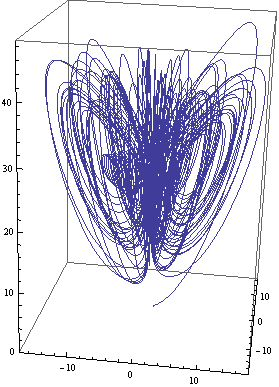
\includegraphics[width=0.35\textwidth]{CLEx1x2z}
\end{center}
\caption{
$\{x_1,x_2,z\}$ plot of 2-mode system, with initial point
$(x_1, x_2, y_1, y_2, z) = (1, 0, 0, 1, 1)$.
    }
\label{fig:2mEx1x2z}
\end{figure}
    } %end solution{exer:2mPlotCLf}

\section{Linear stability}

\exercise{\Stabmat\ of 2-mode system:}{ \label{exer:2mStabmatCLf}
Find the \stabmat\ of 2-mode system\ \refeq{eq:2meR}.
    }

\solution{exer:2mStabmatCLf}{\Stabmat\ of 2-mode system:}{
(solution not available)
    }



\section{Symmetries of dynamics}


\subsection{Rotational equivariance of 2-mode system}

\exercise{\Un{1} equivariance of 2-mode system for finite angles:}{ \label{exer:2mFinRotInvarCmplx}
Show that 2-mode system \refeq{eq:2me} is equivariant under rotation for finite angles.
    }

\solution{exer:2mFinRotInvarCmplx}{\Un{1} equivariance of \cLe\ for finite angles.}{
Obvious by inspection; that's how the equations \refeq{eq:2me}
were constructed in the first place.}

\exercise{\SOn{2} equivariance of the 2-mode system for finite angles:}{ \label{exer:2mFinRotInvari}
Show that the 2-mode system is equivariant under rotation for finite angles.
    }

\solution{exer:2mFinRotInvari}{\SOn{2} equivariance of the 2-mode system for finite angles.}{
(solution not available)
    }

\exercise{\SOn{2} equivariance of the 2-mode system for infinitesimal angles.}
   { \label{exer:2mInfinRotInvari}
Show that the 2-mode system is equivariant under rotation for infinitesimal angles.
    }

\solution{exer:2mInfinRotInvari}
         {\SOn{2} equivariance of the 2-mode system for infinitesimal angles.}{
We can
 check the equivariance condition \refeq{eq:InfnmslRot},
$0=- \Lg v(x)+\Mvar \Lg x$,
where $\Mvar=\frac{\pde v}{\pde x}$ is the \stabmat, by explicit substitution.
The matrix $ \Lg $ is
\beq
 \Lg =\left(\barr{ccccc}
0&1&0&0&0\\
-1&0&0&0&0\\
0&0&0&2&0\\
0&0&-2&0&0\\
0&0&0&0&0
\earr\right)
\,.
\ee{SO2gener2me}
Plugging these into \refeq{eq:InfnmslRot} and using
\refeq{eq:2meR} for $v(x)$ should yield a zero vector.
    \PC{9 Jul 2009 - have not checked this}.
    } % end \solution{exer:2mInfinRotInvari}

\exercise{Discover the equivariance of a given flow:}{ \label{exer:discvInvar}
Suppose you were given \cLe, but nobody told you they are \SOn{2} equivariant.
More generally, you might encounter a flow without realizing that it
has a continuous symmetry - how would you test for it?
    }

\solution{exer:discvInvar}{Discover the equivariance of a given flow?}{
If $M$ is in the Lie algebra, by the equivariance condition \refeq{eq:InfnmslRot}
the Lie derivative
$
M \cdot v(x)-\Mvar \cdot M \cdot \ssp
$
vanishes. You have $v(x)$ and the \stabmat\ $\Mvar$, hence try finding whether
a $M$ can be found such that the Lie derivative vanishes. You know that if the
symmetry group is a subgroup of \SOn{d}, the Lie algebra elements $M$ can be
taken antisymmetric. (Have not tried to solve
this problem, so let us know if you succeed)
\authorPC{Aug 25 2009}
    }

\section{\Eqva}

An \eqv\ is any point for which the velocity
field of an ordinary differential equation is zero.

\exercise{\Eqva\ of 2-mode system:}{\label{exer:2mEquiCLe}
Find all \eqva\ of 2-mode system.
    }

\solution{exer:2mEquiCLe}{\Eqva\ of 2-mode system.}{
(solution not available)
    } %end \solution{exer:2mEquiCLe}{\Eqva\ of 2-mode system.}

\section{\Reqva}

\subsection{Equations in the polar form}

\exercise{2-mode system in polar coordinates.}{\label{exer:2mpolarCLe}
Rewrite 2-mode system from Cartesian to polar coordinates,
\beq
(x_1,x_2,y_1,y_2,z) =
    (\rho_1 \cos\theta_1,\rho_1\sin\theta_1,
     \rho_2\cos\theta_2,\rho_2\sin\theta_2,z)
\,,
\label{eq:2mCartToPol}
\eeq
where $\rho_1 \geq 0 \,,\rho_2 \geq 0$.
    }

\solution{exer:2mpolarCLe}{2-mode system in polar coordinates.}{
(solution not available)
} % end \solution{exer:2mpolarCLe}{2-mode system in polar coordinates

\subsection{Computing and plotting the relative equilibrium $Q_1$}

\exercise{Computing the \reqv\ $Q_1$:}{\label{exer:2mCompRelEqu}
Find the \reqva\ of the 2-mode system by finding the \eqva\ of the
system in polar coordinates \refeq{eq:PolarCLeTheta}.
}

\solution{exer:2mCompRelEqu}{Computing the \reqv\  $Q_1$.}{
(solution not available)
} % end \solution{exer:2mCompRelEqu}{Computing the Relative Equilibrium $Q_1$

\exercise{Plotting \reqv\ $\REQB{1}$ in polar coordinates:}{\label{exer:2mPlotPolEqu}
Plot the equilibrium $\REQB{1}$ in polar coordinates.
}

\solution{exer:2mPlotPolEqu}{Plotting \reqv\ $\REQB{1}$ in polar coordinates.}{
(solution not available)
} % end \solution{exer:2mPlotPolEqu}{Plotting the Relative Equilibrium $\REQB{1}$ in Polar Coordinates

\exercise{Plotting \reqv\ $\REQB{1}$ in Cartesian coordinates:}{\label{exer:2mPlotRelEqu}
Plot the relative equilibrium $\REQB{1}$ in Cartesian coordinates.
}

\solution{exer:2mPlotRelEqu}{Plotting \reqv\ $\REQB{1}$ in Cartesian coordinates.}{
(solution not available)
} % end \solution{exer:2mPlotRelEqu}{Plotting the Relative Equilibrium $\REQB{1}$ in Cartesian

\subsection{Eigenvalues and eigenvectors of the \stabmat}

\exercise{Eigenvalues and eigenvectors of $\EQV{0}$ \stabmat:}
         {\label{exer:2mEigenE0}
Find the eigenvalues and the eigenvectors of the \stabmat\ $\Mvar$ at $\EQV{0}$.
}

\solution{exer:2mEigenE0}{Eigenvalues and eigenvectors of $\EQV{0}$ \stabmat.}{
(solution not available)
} % end \solution{exer:2mEigenE0}{eigenvectors of $\EQV{0}$ \stabmat

\exercise{Plotting the eigenvalues and eigenvectors of the \stabmat\ at $\EQV{0}$:}{\label{exer:2mPlotEigenE0}
Plot the eigenvectors of $\Mvar$ at $\EQV{0}$ and the 2-mode
system at values very close to $\EQV{0}$.
}

\solution{exer:2mPlotEigenE0}
{Plotting the eigenvalues and eigenvectors of the \stabmat\ at $\EQV{0}$:}{
(solution not available)
} % end \solution{exer:2mPlotEigenE0}{Plotting the eigenvalues and eigenvectors of the stability matrix at $\EQV{0}$

\exercise{Finding the eigenvalues and eigenvectors of  $\REQB{1}$ \stabmat:}{\label{exer:2mEigenE0}
Compute the eigenvalues and eigenvectors of the stability
matrix evaluated at $\REQB{1}$ and using the Siminos thesis
values \refeq{SiminosPrmts}.
}

\solution{exer:2mEigenE0}{Finding the eigenvalues and eigenvectors of  $\REQB{1}$ \stabmat.}{
(solution not available)
} % end \solution{exer:2mEigenE0}{Finding the eigenvalues and eigenvec

\exercise{Plotting the eigenvalues and eigenvectors of
the stability matrix at $\REQB{1}$ in polar coordinates:}{\label{exer:2mPlotPolEigenQ1}
Plot the eigenvectors of \Mvar\ at $\REQB{1}$ in polar
coordinates, as well as the polar 2-mode system at values very near
$\REQB{1}$.
}

\solution{exer:2mPlotPolEigenQ1}{Plotting the eigenvalues and eigenvectors of
the stability matrix at $\REQB{1}$ in polar coordinates.}{
(solution not available)
} % end \solution{exer:2mPlotPolEigenE1}{Plotting the eigenvalues
